
\subsubsection{フロアマップを用いた歩行可能座標への補正}

図\ref{fig:pdr-rotate}に示す軌跡には,人間が歩行可能座標ではない場所を
通過している問題ある.図\ref{fig:walkable-points}は
ある軌跡上の点が歩行可能な座標であるか否かを示している.青色の点は
歩行可能な座標上に存在する点を,赤色の点は歩行不可能な座標上に
存在する点を表している.この図から分かるように,軌跡の一部が壁や
障害物の存在する座標を通過している.このような軌跡は人間の実際の
歩行経路としては物理的に不適切である.この問題に対処するため,
本ライブラリではMapMatchCorrectorクラスの歩行可能座標補正機能を提供している.

\begin{figure}[H]
    \centering
    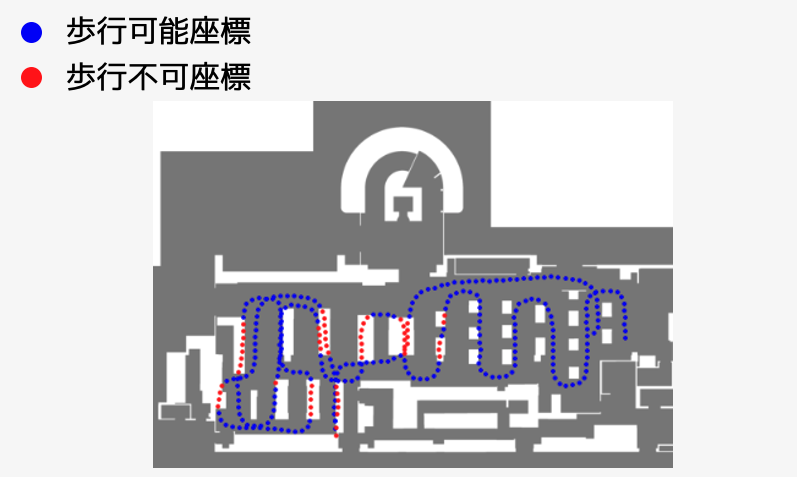
\includegraphics[width=\linewidth]{../image/unwalkable_points.jpg}
    \caption{}    \label{fig:unwalkable_points}
\end{figure}

この手法を利用するために必要な情報は,前節と同様のフロアマップ情報である.
このマップ情報を用いて,軌跡上の各点が歩行可能な座標に存在するように
補正を行う.
% TODO 2.前の項で出したマップマッチングとの関係性についても触れてもいいのかもしれない,
% こちらはより詳細なマップマッチングな気がする?

補正処理は以下の手順で行われる.まず,軌跡上の各点について,その座標が
フロアマップ上の歩行可能座標に存在するかを判定する.ある時刻$t$の
座標$(x_t, y_t)$が歩行不可能な座標に存在する場合,その点からもっとも近い
歩行可能な座標$(x_t^*, y_t^*)$を探索する.

この探索には幅優先探索(BFS)アルゴリズムを用いる.具体的には,現在の
座標から上下左右および斜め方向に探索を行い,最初に見つかった歩行可能な
座標を$(x_t^*, y_t^*)$として採用する.この際,探索はマップの境界を
超えないように制限される.

歩行可能な座標が見つかった場合,時刻$t$以降の全ての軌跡の座標を,
以下の式に従って平行移動する.

\begin{equation}
x_k' = x_k + (x_t^* - x_t), \quad y_k' = y_k + (y_t^* - y_t) \quad (k \geq t)
\end{equation}

ここで,$(x_k', y_k')$は補正後の座標,$(x_k, y_k)$は補正前の座標を表す.
この処理により,歩行不可能座標に存在していた点とそれ以降の軌跡が,
もっとも近い歩行可能な座標へと移動される.

この補正処理は軌跡の始点から順に適用される.図\ref{fig:map-matching}に
示すように,補正後の軌跡では全ての点が歩行可能な座標内に存在している.

なおこの補正処理は前節までの補正とは異なり,軌跡の進行方向は保持
したまま,位置のみを補正する特徴がある.
% TODO:2.この処理をしても壁抜けは防げないのを説明した方がいいかもしれない
\begin{figure}[H]
    \centering
    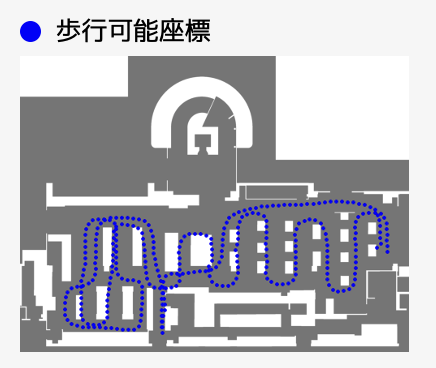
\includegraphics[width=\linewidth]{../image/walkable-points.jpg}
    \caption{マップマッチング補正後の軌跡}    \label{fig:walkable-points}
\end{figure}
